\documentclass[8pt,landscape,a4paper]{article}
\usepackage[utf8x]{inputenc}
\usepackage[french]{babel}
\usepackage[T1]{fontenc}
\usepackage{tikz}
\usetikzlibrary{shapes,positioning,arrows,fit,calc,graphs,graphs.standard}
\usepackage[nosf]{kpfonts}
\usepackage[t1]{sourcesanspro}
\usepackage{multicol}
\usepackage{wrapfig}
\usepackage[top=1cm,bottom=1cm,left=1cm,right=1cm]{geometry}
\usepackage[framemethod=tikz]{mdframed}
\usepackage{microtype}
\usepackage{pdfpages}
\usepackage{lipsum} 
\usepackage{array} 

\let\bar\overline

\definecolor{myblue}{rgb}{0.28,0.0,1.0}

\def\firstcircle{(0,0) circle (1.5cm)}
\def\secondcircle{(0:2cm) circle (1.5cm)}

\colorlet{circle edge}{myblue}
\colorlet{circle area}{myblue!5}

\tikzset{filled/.style={fill=circle area, draw=circle edge, thick},
    outline/.style={draw=circle edge, thick}}
    
\pgfdeclarelayer{background}
\pgfsetlayers{background,main}

% \everymath\expandafter{\the\everymath \color{myblue}}
% \everydisplay\expandafter{\the\everydisplay \color{myblue}}

\renewcommand{\baselinestretch}{.8}
\pagestyle{empty}

\global\mdfdefinestyle{header}{%
linecolor=gray,linewidth=1pt,%
leftmargin=0mm,rightmargin=0mm,skipbelow=0mm,skipabove=0mm,
}

\newcommand{\header}{
\begin{mdframed}[style=header]
\footnotesize
\sffamily
\textbf{Vim Cheatsheet}\\
{\scriptsize sebastien.druon@umontpellier.fr}
\end{mdframed}
}

\makeatletter % Author: https://tex.stackexchange.com/questions/218587/how-to-set-one-header-for-each-page-using-multicols
\renewcommand{\section}{\@startsection{section}{1}{0mm}%
                                {.7ex}%
                                {.7ex}%x
                                {\color{myblue}\sffamily\small\bfseries}}
\renewcommand{\subsection}{\@startsection{subsection}{1}{0mm}%
                                {.7ex}%
                                {.7ex}%x
                                {\sffamily\bfseries}}

\def\multi@column@out{%
   \ifnum\outputpenalty <-\@M
   \speci@ls \else
   \ifvoid\colbreak@box\else
     \mult@info\@ne{Re-adding forced
               break(s) for splitting}%
     \setbox\@cclv\vbox{%
        \unvbox\colbreak@box
        \penalty-\@Mv\unvbox\@cclv}%
   \fi
   \splittopskip\topskip
   \splitmaxdepth\maxdepth
   \dimen@\@colroom
   \divide\skip\footins\col@number
   \ifvoid\footins \else
      \leave@mult@footins
   \fi
   \let\ifshr@kingsaved\ifshr@king
   \ifvbox \@kludgeins
     \advance \dimen@ -\ht\@kludgeins
     \ifdim \wd\@kludgeins>\z@
        \shr@nkingtrue
     \fi
   \fi
   \process@cols\mult@gfirstbox{%
%%%%% START CHANGE
\ifnum\count@=\numexpr\mult@rightbox+2\relax
          \setbox\count@\vsplit\@cclv to \dimexpr \dimen@-1cm\relax
\setbox\count@\vbox to \dimen@{\vbox to 1cm{\header}\unvbox\count@\vss}%
\else
      \setbox\count@\vsplit\@cclv to \dimen@
\fi
%%%%% END CHANGE
            \set@keptmarks
            \setbox\count@
                 \vbox to\dimen@
                  {\unvbox\count@
                   \remove@discardable@items
                   \ifshr@nking\vfill\fi}%
           }%
   \setbox\mult@rightbox
       \vsplit\@cclv to\dimen@
   \set@keptmarks
   \setbox\mult@rightbox\vbox to\dimen@
          {\unvbox\mult@rightbox
           \remove@discardable@items
           \ifshr@nking\vfill\fi}%
   \let\ifshr@king\ifshr@kingsaved
   \ifvoid\@cclv \else
       \unvbox\@cclv
       \ifnum\outputpenalty=\@M
       \else
          \penalty\outputpenalty
       \fi
       \ifvoid\footins\else
         \PackageWarning{multicol}%
          {I moved some lines to
           the next page.\MessageBreak
           Footnotes on page
           \thepage\space might be wrong}%
       \fi
       \ifnum \c@tracingmulticols>\thr@@
                    \hrule\allowbreak \fi
   \fi
   \ifx\@empty\kept@firstmark
      \let\firstmark\kept@topmark
      \let\botmark\kept@topmark
   \else
      \let\firstmark\kept@firstmark
      \let\botmark\kept@botmark
   \fi
   \let\topmark\kept@topmark
   \mult@info\tw@
        {Use kept top mark:\MessageBreak
          \meaning\kept@topmark
         \MessageBreak
         Use kept first mark:\MessageBreak
          \meaning\kept@firstmark
        \MessageBreak
         Use kept bot mark:\MessageBreak
          \meaning\kept@botmark
        \MessageBreak
         Produce first mark:\MessageBreak
          \meaning\firstmark
        \MessageBreak
        Produce bot mark:\MessageBreak
          \meaning\botmark
         \@gobbletwo}%
   \setbox\@cclv\vbox{\unvbox\partial@page
                      \page@sofar}%
   \@makecol\@outputpage
     \global\let\kept@topmark\botmark
     \global\let\kept@firstmark\@empty
     \global\let\kept@botmark\@empty
     \mult@info\tw@
        {(Re)Init top mark:\MessageBreak
         \meaning\kept@topmark
         \@gobbletwo}%
   \global\@colroom\@colht
   \global \@mparbottom \z@
   \process@deferreds
   \@whilesw\if@fcolmade\fi{\@outputpage
      \global\@colroom\@colht
      \process@deferreds}%
   \mult@info\@ne
     {Colroom:\MessageBreak
      \the\@colht\space
              after float space removed
              = \the\@colroom \@gobble}%
    \set@mult@vsize \global
  \fi}

\makeatother
\setlength{\parindent}{0pt}

\begin{document}
\small

\begin{multicols*}{3}

    \section{Launching ... and exiting}

    \subsection{invocation}

    \begin{tabular}{m{7cm} l}
        \texttt{vim file1 file2 ... fileN}   & \\
        \texttt{vim +linenumber file}  & \\
        \texttt{vim scp://login@serveur/path/to/file}  & \\
        \texttt{vim scp://login@serveur/path/}  & \\
    \end{tabular}

    \subsection{Exiting}
    \begin{tabular}{m{2cm} l}
        \texttt{:q}   & Quit\\
        \texttt{:qa}  & Close all files\\
        \texttt{:wq}  & Save and quit \\
        \texttt{:q!}  & Quit without saving\\
    \end{tabular}

    \section{Moving}
    \begin{tabular}{m{2cm} l}
        \texttt{h,j,k,l}  & Move cursor \\
        $\leftarrow$ $\downarrow$ $\uparrow$ $\rightarrow$  & Move cursor \\
    \end{tabular}
    
    \subsection{Inside the line}
    \begin{tabular}{m{2cm} l}
        \texttt{0}  & Jump to first char \\
        \texttt{\$} & Jump to last char \\
        \texttt{\^} & Jump to first word of the line \\
        \texttt{w}  & Next word\\
        \texttt{b}  & Previous word\\
        \texttt{f char} & Jump to next occurence of char \\
        \texttt{t char} & Jump before next occurence of char \\
        \texttt{F char} & Jump to previous occurence of char \\
        \texttt{T char} & Jump after previous occurence of char \\
        \texttt{;} & Repeat last f/t command \\
        \texttt{,} & Repeat last F/T command \\
    \end{tabular}
    
    \subsection{Inside the file }
    \begin{tabular}{m{2cm} l}
        \texttt{gg} & Jump to first line (start)\\
        \texttt{G}  & Jump to last line (start) \\
        \texttt{nnn gg} & Jump to line nnn \\
        \texttt{\%} & Jump to matching Paren, Brace, etc. \\
    \end{tabular}

    \subsection{Inside the screen}
    \begin{tabular}{m{2cm} l}
        \texttt{zz} & Center the current line \\
        \texttt{zb} & Send current line to the bottom \\
        \texttt{zt} & Send current line to the top \\
        \texttt{H} & Jump to the top of the file \\
        \texttt{M} & Jump to the middle of the file \\
        \texttt{L} & Jump to the bottom of the file \\
        \texttt{CTRL + b} & Scroll up \\
        \texttt{CTRL + u} & Scroll up (half a page)\\
        \texttt{CTRL + d} & Scroll down (half a page) \\
        \texttt{CTRL + f} & Scroll down \\
    \end{tabular}

    \section{Switch to insert mode}
    \begin{tabular}{m{2cm} l}
        \texttt{i}  & At cursor position\\
        \texttt{a}  & After cursor\\
        \texttt{A}  & At the end of the line\\
        \texttt{o}  & Open a new line (after)\\
        \texttt{O}  & Open a new line (before)\\
    \end{tabular}
    
    \section{Switch to visual mode}
    \begin{tabular}{m{2cm} l}
        \texttt{v}& Visual mode (char by char)\\
        \texttt{V}& Visual mode (line by line)\\
        \texttt{CTRL+v}& Visual mode (block)\\
    \end{tabular}

    \section{Normal mode}
    \begin{tabular}{m{2cm} l}
        \texttt{u}& Undo\\
        \texttt{CTRL+r}& Redo\\
        \texttt{.}& Repeat last edit\\
    \end{tabular}\\

    \section{Without leaving Insert mode}
    \begin{tabular}{m{2cm} l}
        \texttt{CTRL+w} & Erase previous word\\
        \texttt{CTRL+u} & Erase until the begining of the line\\
        \texttt{CTRL+o} & Single command mode command\\
    \end{tabular}\\

    \section{Open / Save}
    \begin{tabular}{m{2cm} l}
        \texttt{:e fichier}& Open a file in a buffer\\
        \texttt{:w}& Save\\
        \texttt{:w fichier}& Save as \\
        \texttt{:browse old}& Recently opened file \\

    \end{tabular}\\
    \section{Buffers}
    \begin{tabular}{m{2cm} l}
        \texttt{:ls}& List all buffers\\
        \texttt{:b7}& Switch to buffer 7\\
        \texttt{:bn}& Next buffer\\
        \texttt{:bp}& Previous buffer\\
    \end{tabular}\\

    \section{Windows}
    \begin{tabular}{m{4cm} l}
        \texttt{CTRL+w v}& Split vertically\\
        \texttt{CTRL+w s}& Split horizontally\\
        \texttt{CTRL+w h,j,k,l }& Change window\\
        \texttt{CTRL+w H,J,K,L }& Move window\\
        \texttt{CTRL+w R,r }& Rotate windows\\
        \texttt{CTRL+w c }&Close window\\
    \end{tabular}\\

    Of course, you can substitute h,j,k,l by arrows \\
        
    \begin{tabular}{m{3cm} l}
	\texttt{:sp file}& Open file in a split window\\
    \end{tabular}\\
    
    \section{Sessions}
    \begin{tabular}{m{4cm} l}
        \texttt{:mks fichier.vim} & Save the session\\
        \texttt{:source fichier.vim} & Restore the session\\
    \end{tabular}\\

    \section{Search}
    \begin{tabular}{m{2cm} l}
        \texttt{/word}& Find next occurence of "word"\\
        \texttt{?word}& Find last occurence of "word"\\
        \texttt{n}& Next\\
        \texttt{N}& Previous\\
    \end{tabular}
    
    \section{ Macros }
    \begin{tabular}{m{2cm} l}
        \texttt{qa} & Record macro a\\
        \texttt{q} & Stop recording macro\\
        \texttt{@a} & Run macro a\\
        \texttt{@@} & Rerun last run macro\\
    \end{tabular}\\
    
    \section{Copy / Paste}
    \subsection{ Copy current selection }
    \begin{tabular}{m{2cm} l}
        \texttt{y}& (yank) Copy\\
        \texttt{d}& (delete) Cut\\
    \end{tabular}
    \subsection{ Paste }
    \begin{tabular}{m{2cm} l}
        \texttt{p}& (put) Paste (after)\\
        \texttt{P}& (put) Paste (before)\\
    \end{tabular}
    \subsection{ Copy without selection selection }
    \begin{tabular}{m{2cm} l}
        \texttt{yy}& Copy current line\\
        \texttt{dd}& Cut current line\\
        \texttt{yny}& Copy n lines \\
        \texttt{yw}& Copy current word\\
        \texttt{y\$}& Copy from cursor to the end of the line\
    \end{tabular}

    \subsection{ Using registers }
    \begin{tabular}{m{2cm} l}
        \texttt{"ay}& Copy in register a\\
        \texttt{"Ay}& Copy and add to a register\\
        \texttt{:reg}& Display registers\\
    \end{tabular} \\

    The registers you can use are the following :\\

    \begin{tabular}{m{2cm} l}
        \texttt{a..z}& 26 general-purpose registers\\
        \texttt{1..9}& 9 last uses of d\\
        \texttt{+}   & System copy-paste register (ctrl+c)\\
        \texttt{*}   & System copy-paste register (mouse)\\
        \texttt{\%}  & Filename\\
    \end{tabular} \\


    \section{Search \& replace}
    
    \texttt{:\%s{\char`\/}expr1/expr2/g} \\
    
    \begin{tabular}{m{2cm} l}
        \texttt{expr1 }   &  Expression we're searching \\
        \texttt{expr2 }   &  Replacement expression\\
        \texttt{\% }   &  Search scope\\
        \texttt{g }   &  Options\\
    \end{tabular}\\

    \subsection{Scope:}
    \begin{tabular}{m{2cm} l}
        \texttt{n,m}  & From line n to m\\
        \texttt{.,+5} & Current line and 5 following \\
        \texttt{\%}   & In all file\\
    \end{tabular}\\

    \subsection{Options:}
    \begin{tabular}{m{2cm} l}
        \texttt{g} & Continue after first match\\
        \texttt{c} & Ask before replacing\\
        \texttt{i} & Ignore case\\
    \end{tabular}\\
    
    \subsection{Replace with foobar (y/n/a/q/l/\^{}E/\^{}Y) ?}
    \begin{tabular}{m{2cm} l}
        \texttt{y} & Yes\\
        \texttt{n} & No\\
        \texttt{a} & Replace all remaining matches\\
        \texttt{q} & Quit substitution\\
        \texttt{l} & Last one !\\
        \texttt{CTRL + e} & Scroll down\\
        \texttt{CTRL + y} & Scroll up \
    \end{tabular}\\
    
    \section{ Marking lines }
    \begin{tabular}{m{2cm} l}
        \texttt{m a} & Mark line in register a\\
        \texttt{' a} & Return to mark a\\
    \end{tabular}\\
    
    \section{Shell Commands}
    \begin{tabular}{m{2cm} l}
        \texttt{:r file} & Insert the content of <file> \\
        \texttt{:! cmd}  & Execute the command cmd in a shell\\
        \texttt{:r! cmd} & Execute the command cmd and insert the result \\
        \texttt{:term} & Open a terminal window \\
    \end{tabular}\\

    \section{ Tabs }
    \begin{tabular}{m{2cm} l}
        \texttt{:tabnew} & Open a new tab\\
        \texttt{gt} & Move to next tab\\
        \texttt{gT} & Move to previous tab\\
        \texttt{:tab ba} & Edit all buffers as tabs\\
    \end{tabular}\\
    
    \section{Spell checking}
    \begin{tabular}{m{4cm} l}
        \texttt{:spell lang=fr} & Start spell checking\\
        \texttt{:setlocal spell lang=fr} & Correction in current buffer\\
        \texttt{:set nospell} & Stop spell checking\\
        \texttt{]s} & Next erroneous word\\
        \texttt{[s} & Previous erroneous word\\
        \texttt{z=} & Suggest a correction\\
        \texttt{zg} & Add to dictionary\\
        \texttt{zw} & Mark word as incorrect\\
    \end{tabular}\\

    \section{Coders' corner}
    \subsection{Increase / Decrease}
    \begin{tabular}{m{2cm} l}
        \texttt{CTRL+a} & Adds 1 to a number\\
        \texttt{CTRL+x} & Subsracts 1 to a number\\
    \end{tabular}\\
    \subsection{Indentation}
    \begin{tabular}{m{2cm} l}
        \texttt{=}  & Auto. indent selection\\
        \texttt{==} & Auto. indent line \\
        \texttt{$>$}  & Increase indentation \\
        \texttt{$<$}  & Reduce indentation \\
        \texttt{$>>$} & Increase indentation of the current line\\
        \texttt{$<<$} & Reduce indentation of the current line\\
        \texttt{$n>>$} & Increase by 1 indentation of n lines\\
    \end{tabular}\\
    \subsection{Compilation}
    \begin{tabular}{m{2cm} l}
        \texttt{:make}  & Launch make in the current folder\\
    \end{tabular}\\

    \section{File management (netrw) }
    \begin{tabular}{m{2cm} l}
        \texttt{:Explore} & Open file manager\\
    \end{tabular}\\
    \subsection{ Operations}
    \begin{tabular}{m{2cm} l}
        \texttt{D} & Delete file/directory\\
        \texttt{d} & Create new folder\\
        \texttt{\%} & Open a new file\\
    \end{tabular}\\
    \subsection{ Marked / unmark}
    \begin{tabular}{m{2cm} l}
        \texttt{mf} & Mark a file\\
        \texttt{mu} & Unmark all files\\
        \texttt{mp} & Display marked files\\
        \texttt{mt} & Tag current folder\\
    \end{tabular}\\
    \subsection{ Operations on tagged files}
    \begin{tabular}{m{2cm} l}
        \texttt{me} & Edit\\
        \texttt{md} & Diff\\
        \texttt{mc} & Copy in tagged folder\\
        \texttt{mm} & Move to tagged folder\\
    \end{tabular}\\

    \section{More on windows }

    \subsection{Scroll simultaneously }

    \begin{tabular}{m{3cm} l}
        \texttt{:set scrollbind} & Have windows scroll together\\
    \end{tabular}\\

    \subsection{Resizing windows}

    \begin{tabular}{m{2cm} l}
        \texttt{CTRL-w -} & Decrease the height \\
        \texttt{CTRL-w +} & Increase the height \\
        \texttt{CTRL-w <} & Decrease the width \\
        \texttt{CTRL-w >} & Increase the width \\
        \texttt{CTRL-w =} & Make all splits equal \\
    \end{tabular}\\

    \section{Do you speak vim ?}

    \subsection{ Format }

    <Number of times> + <Command> + <Motion> or <Text object> \\

    \subsection{Commands}
    \begin{tabular}{m{2cm} l}
        \texttt{c} & Change \\
        \texttt{d} & Delete \\
        \texttt{y} & Yank \\
    \end{tabular}\\


    \subsection{Motion}
    \begin{tabular}{m{2cm} l}
        \texttt{)} & Move cursor to end of sentence \\
        \texttt{(} & Move cursor to beginning of prior sentence \\
        \texttt{\}} & Move cursor to the next paragraph \\
        \texttt{\{} & Move cursor to the beginning of the prior paragraph \\
        \texttt{w} & Move cursor to next word \\
        \texttt{b} & Move cursor back a word \\
        \texttt{\$} & Move cursor to the end of the logical line \\
        \texttt{0} & Move cursor to the beginning of the logical line \\
        \texttt{G} & Move cursor to the end of the file \\
        \texttt{gg} & Move cursor to the beginning of the file \\
    \end{tabular}\\

    \subsection{Text Objects}
    
    \begin{tabular}{m{2cm} l}
        \texttt{s} & Sentence \\
        \texttt{w} & Word \\
        \texttt{p} & Paragraph \\
        \texttt{a"} & Quoted string \\
        \texttt{a'} & Quoted string (Single quote)\\
    \end{tabular}\\

    \subsection{More precise Text Objects}

    \begin{tabular}{m{2cm} l}
        \texttt{w}  & From cursor to the end of the word \\
        \texttt{iw} & Inner word (Full word) \\
        \texttt{aw} & Around word (including trailing whitespaces)\\
    \end{tabular}\\
    
    \section{ Digraphs }
    \begin{tabular}{m{2cm} l}
        \texttt{CTRL-k code} & Insert digraph\\
    \end{tabular}\\

	\vfill\null 
	\columnbreak

	\section{ Moves illustrated}

	\vspace{2cm}
	\begin{center}
	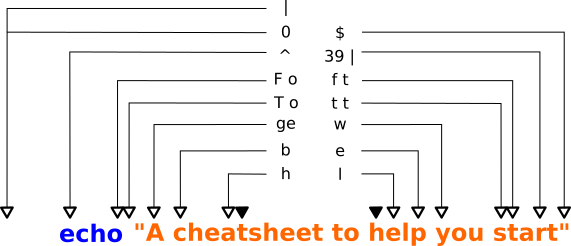
\includegraphics[angle=90,origin=c,scale=0.8]{moves.png}
	\end{center}
	
	\vfill\null 

\end{multicols*}

\end{document}

